%variantes

\section{Variantes}

\subsection{Portable Data File - PDF417}
El código de barras bidimensional PDF417 (Archivo de datos portátil), es el más utilizado y el más antiguos. El código de barras apilado está compuesto por filas de códigos de barras lineales. Siendo bidimensional, le permite llevar más información que los códigos unidimensionales. La razón del número 417, es porque cada patrón o palabra de código codificada en el código de barras está representada por cuatro barras y cuatro espacios. Donde el ancho total de cada palabra de código es de 17 módulos de ancho.
\\
El código de PDF417 empaqueta más información y proporciona redundancia adicional mediante el uso de la técnica de corrección de errores Reed Solomon. Por tal motivo, necesitarán más áreas del código de barras; algunas partes de esa área se utilizarán para la corrección de errores y dará como resultado que se codifiquen menos información. Además, admite diferentes modos de compactación permitiendo que, diferentes tipos de datos sean codificados de manera óptima en el símbolo, por ejemplo, el modo de compactación alfanumérica extendida (EXC) admitiendo la codificación de todos los caracteres ASCII imprimibibles y comprimirlos 2 caracteres por palabra de código.\cite{PDF417Barcode2021}
%496px-PDF417_Example.png
\begin{figure} 
	\centering
	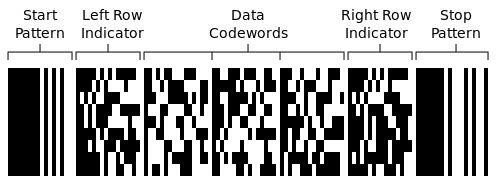
\includegraphics[width=0.7\linewidth]{496px-PDF417_Example.png}
	\caption{Partes de un código o símbolo PDF417. Son omitidas las zonas tranquilas del código.}
	\label{fig:pdf417example}
\end{figure} 

El código PDF417, del desarrollador Symbol Technologies tiene un formato de código de barras apilado. La capacidad de datos varia dependiendo del tipo de datos, para casos númericos 2,710; para alfanúmericos 1,850; binario 1,018 y Kanji 554. Su característica principal es su gran capacidad y sus aplicaciones principales son la automatización de oficinas, licencias de conducir,y también se puede utilizar en los medidores de correo para codificar la cantidad de franqeo, así como en los paquetes de FedEx.\cite{2012_DENSO,2004_FedEx_TECH_REPORT}

\begin{figure} 
	\centering
	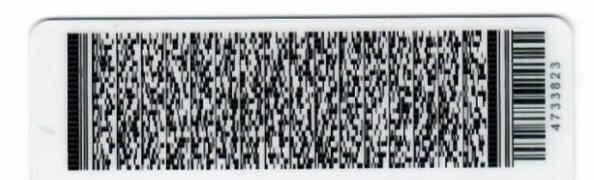
\includegraphics[width=0.7\linewidth]{cedulapdf417.jpg}
	\caption{PDF417 usado en la cédula de identidad (reverso).}
	\label{fig:pdf417CI}
\end{figure} 
\textbf{Ventajas}: Puede codificar cualquier carácter ASCII. Apilar tantos códigos uno encima del otro como desee, permitiendo codificar ilimitada cantidad de datos. Además, para evitar errores, incluye un dígito de control en cada código de barras individual.\cite{cognex.com2021}
\\
\textbf{Desventajas}: Como es posible codificar tanta información como desee en varios códigos apilados, en consecuencia el símbolo crecera de manera proporcional a la cantidad de datos ha codificar.\cite{cognex.com2021}

\subsection{Maxicode}

Maxi Code es un código bidimensional, similar al código unidimensional, pero usa puntos en lugar de barras, con un área de una pulgada al cuadrado, con una diana en el medio, alrededor de ella hay una serie de puntos hexagonaless. También incluye un código de corrección de errores, para que el código se pueda leer incluso si tiene errores o está dañada. Además, de tener varios campos, en los que se codifica el código postal, código de país y código de servicio. También conocido como código Bird's Eye o código UPS.\cite{cognex.com2021}

\begin{figure} 
	\centering
	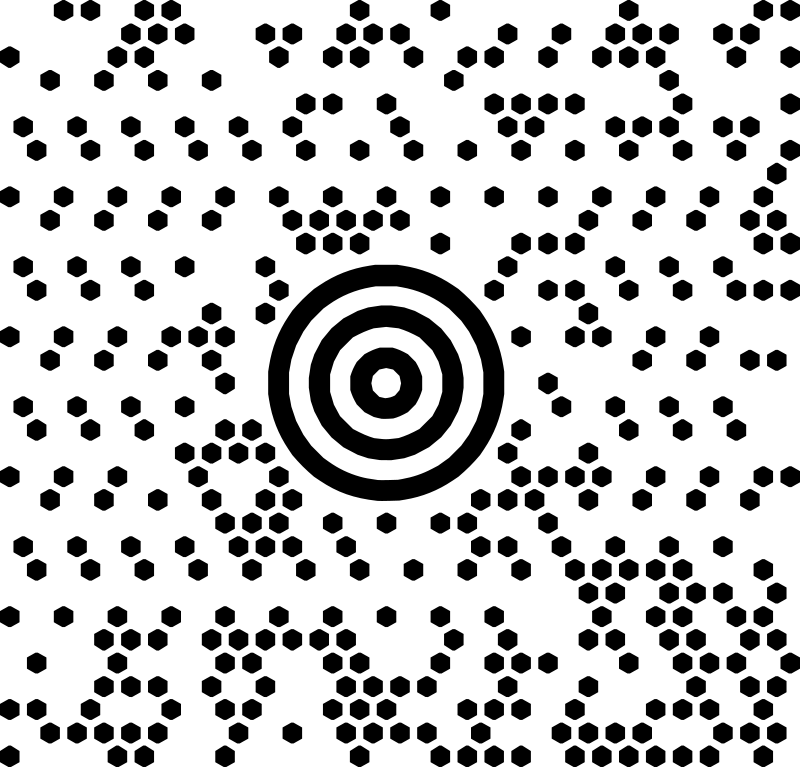
\includegraphics[width=0.2\linewidth]{800px-MaxiCode.svg.png}
	\caption{Ejemplo de un código Maxi.}
	\label{fig:maxicode}
\end{figure} 

El código Maxi, del desarrollador UPS, tiene un formato similar al código QR. La capacidad de datos varia dependiendo del tipo de datos, para casos númericos 138; para alfanúmericos 93; no tiene soporte para tipos de datos binarios y de tipo kanji. Su característica principal es su gran velocidad de lectura y sus aplicaciones principales es en la logística. Se desarrolló originalmente para que lo usara UPS en el seguimiento y envío de paquetes, ya que se puede escanear rápidamente en una cinta transportadora.\cite{2012_DENSO}
\\
\textbf{Ventajas}: escaneo preciso y de forma rápida, incluso en una cinta transportadora en movimiento. \cite{cognex.com2021}
\\
\textbf{Desventajas}: no puede codificar grandes cantidades de información.\cite{cognex.com2021}

\subsection{Datamatrix}

\begin{figure} 
	\centering
	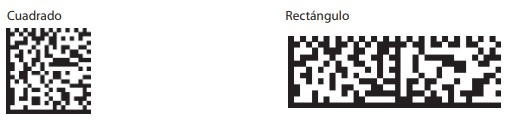
\includegraphics[width=0.5\linewidth]{datamatrix.jpg}
	\caption{Ejemplo de un DataMatrix.}
	\label{fig:DataMatrixRectNormal}
\end{figure}
El código DataMatrix o Matriz de datos, es un código bidimensional, puede tener una configuración cuadrada o rectangular. 
El ECC200 utiliza Reed-Solomon mejorado para la correción de errores eliminado los problemas de distorción, que restaura datos de partes dañadas del símbolo. La tasa de corrección de errores se determina de forma automática dependiendo de la cantidad de datos y el tamaño del símbolo. ECC200 está estandarizado internacionalmente (ISO).\cite{2006_Semacode_TECH_REPORT}

\begin{figure} 
	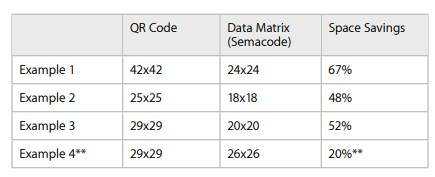
\includegraphics[width=0.6\linewidth]{QRvsDatamatrix.jpg}
	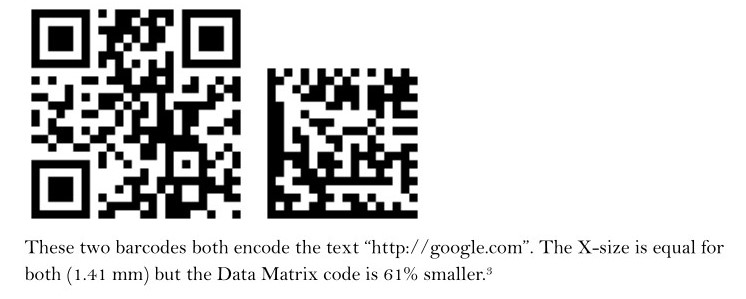
\includegraphics[width=0.6\linewidth]{qrvsdatamatrix2.jpg}
	\caption{Diferencia de espacio entre un código QR y una matriz de datos.(** Caracteres japoneses)}
	\label{fig:datamatrixvsqr}
\end{figure}
En 1989, fue diseñado y estandarizado por socios como la NASA, EE.UU, DoD (U.S. Department of Defense), FDA (Food and Drug Administration) y las industrias como la electronica y el mercado postal. En cambio, QR fue desarrollado en 1994, y su característica distintiva, codificar los caracteres kana japoneses (Kanji).\cite{2006_Semacode_TECH_REPORT}
Pero debido a su pequeño tamaño, existe la dificultad de lectura dado por el enfoque del lector. Por está razón, queda relegado a uso industrial con lectores o escaners especializados. 
\\
El código de matriz de datos, del desarrollador RVSI ACuity CiMatrix, tiene un formato de tipo matricial. La capacidad de datos varia dependiendo del tipo de datos, para casos númericos 3,116; para alfanúmericos 2,355; binario 1,556. Su caraterística principal es su tamaño pequeño y sus aplicaciones principales son la automatización industrial, fabricación de almacenaje, sector sanitario. \cite{2012_DENSO}
\begin{figure} 
%\centering
	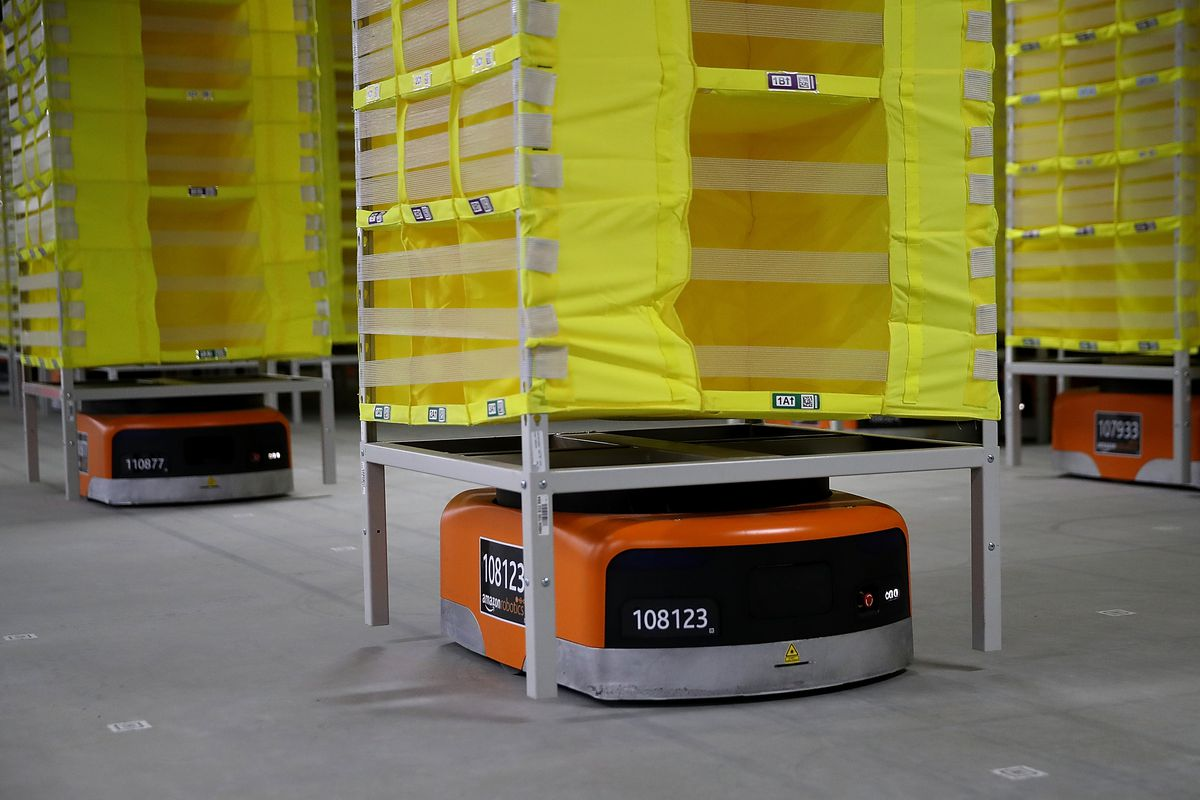
\includegraphics[width=0.5\linewidth]{829377014.jpg.0.jpg}
	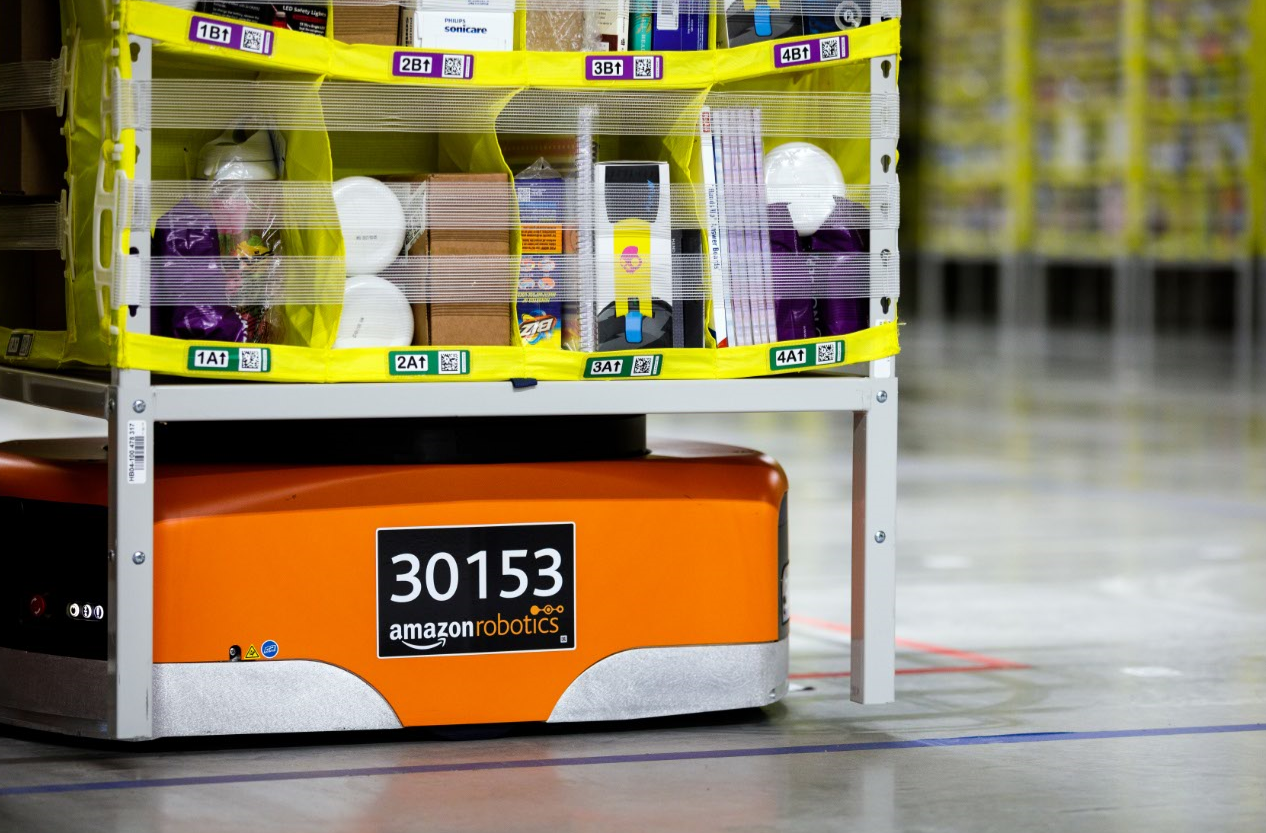
\includegraphics[width=0.5\linewidth]{amazon-robot.png}
	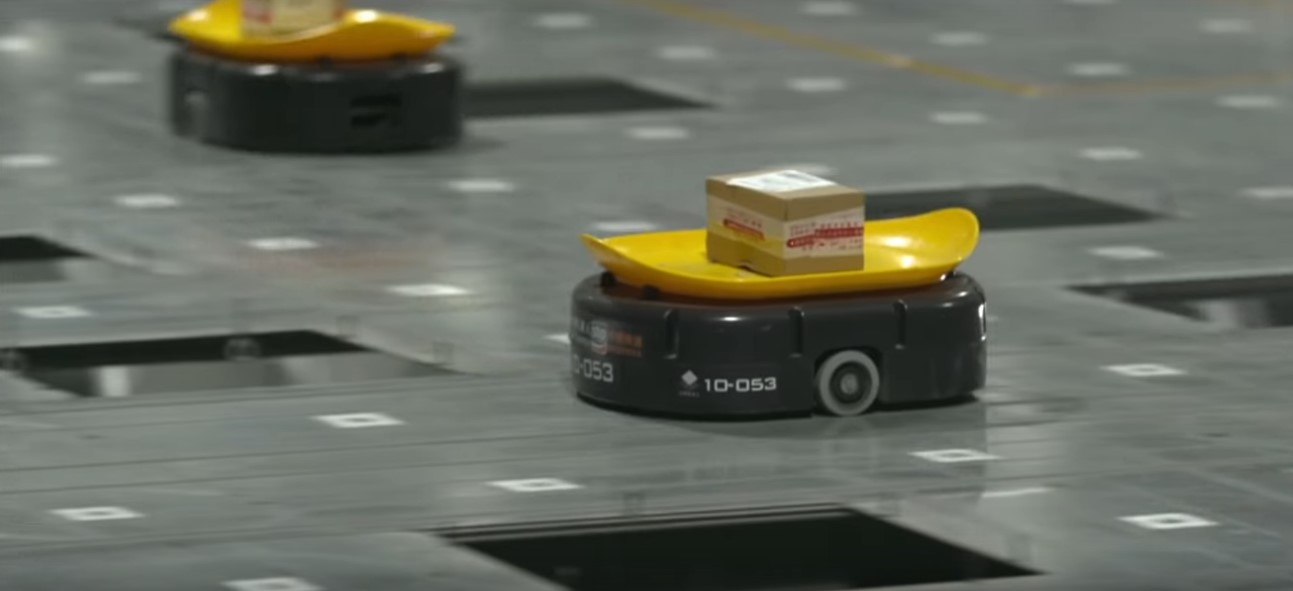
\includegraphics[width=0.5\linewidth]{robotQR.jpg}
	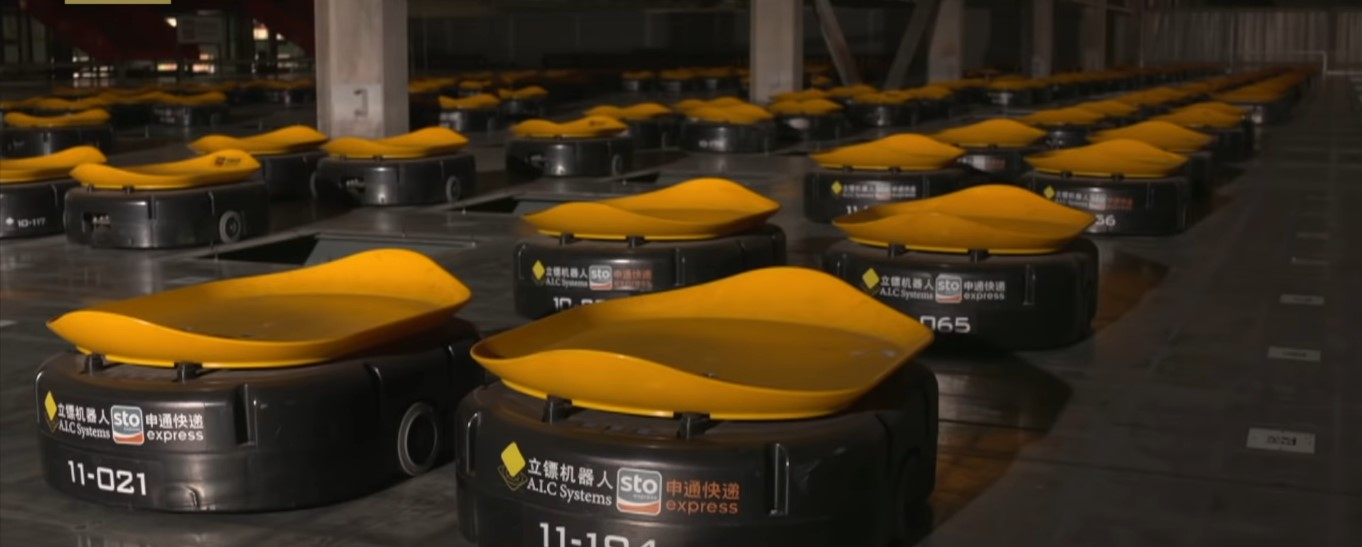
\includegraphics[width=0.5\linewidth]{qrRobot.jpg}
	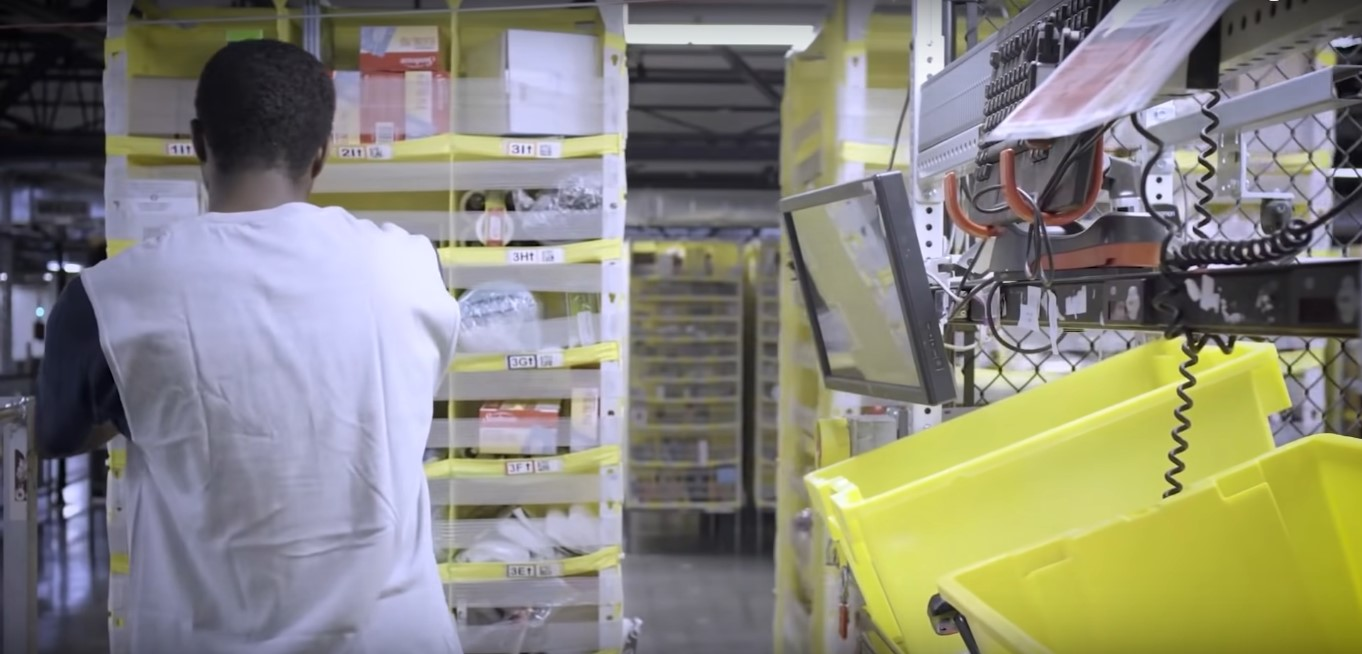
\includegraphics[width=0.5\linewidth]{AmazonSmartWarehouse.jpg}
	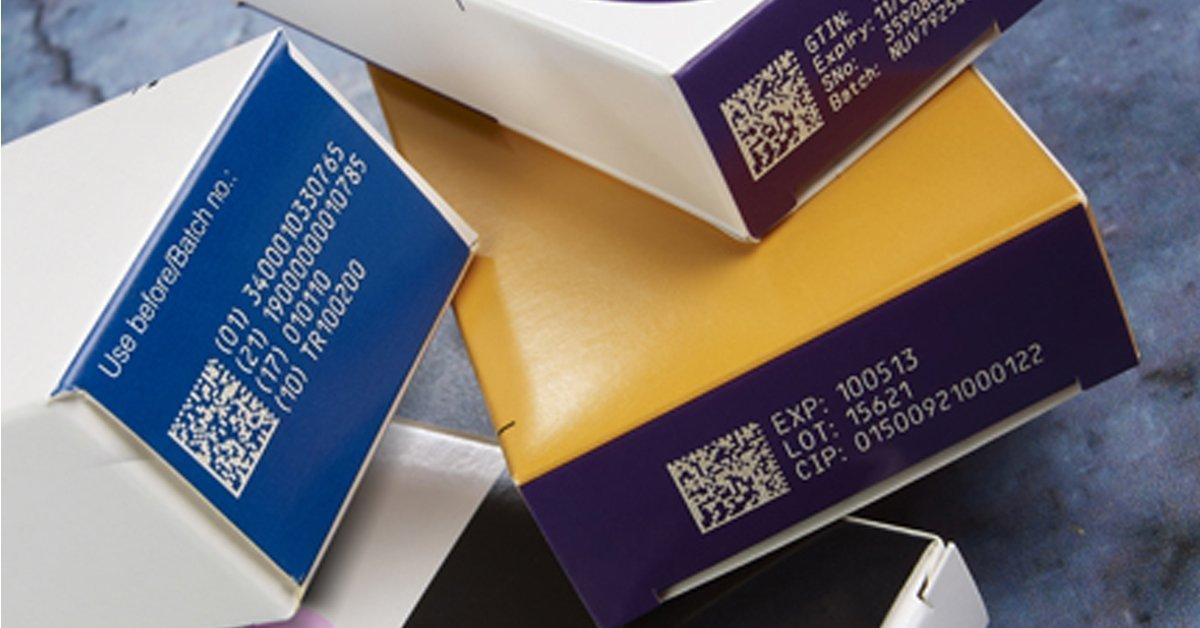
\includegraphics[width=0.5\linewidth]{medicinadatamatrix.jpg}
	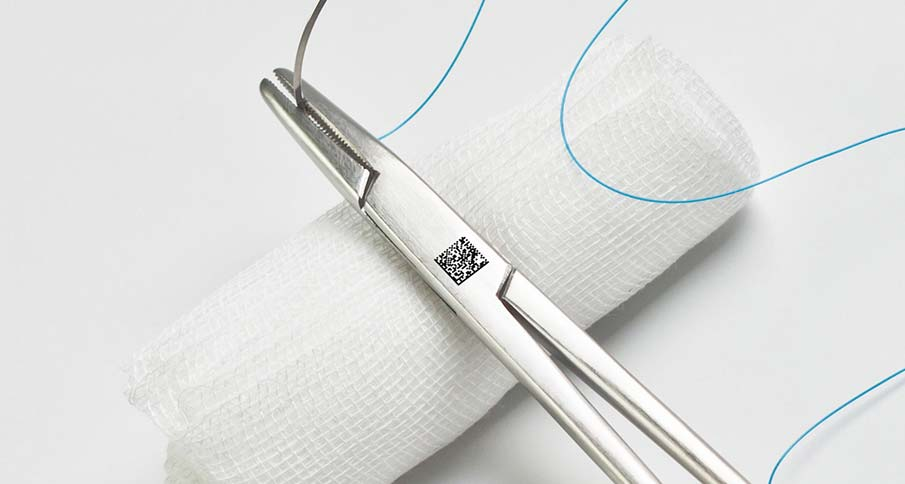
\includegraphics[width=0.5\linewidth]{datamatrixherramientas.jpg}
	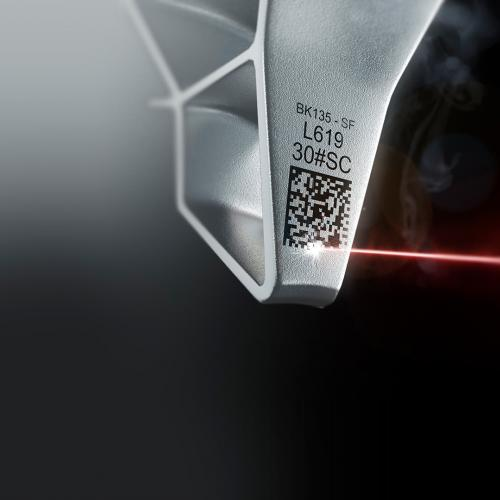
\includegraphics[width=0.3\linewidth]{banner-mkt-a-laser-datamatrix-3d.jpg}
	\caption{Ejemplo de Usos del DataMatrix.}
	\label{fig:datamatrixaplicaciones}
\end{figure}
\newpage
\textbf{“Data Matrix has proven to be the most space efficient of all the twodimensional symbologies.”}
- Consumer Electronics Association’s R9 Automatic Data Capture group (Comparando QR con DataMatrix)\cite{2006_Semacode_TECH_REPORT}
\\
Vea la figura (\ref{fig:datamatrixaplicaciones}), se incluye algunas aplicaciones del código datamatrix, uno de ellos es el uso en los medicamentos o en instrumentos de cirugías por su tamaño y en otros para identificar auto partes (mediante el grabado en metal). En cambio, es también utilizado para automatizar la entrega de los productos, el código es colocado en el suelo; donde los robots se mueven ubicando su posición mediante la lectura del símbolo, complementando con el uso de la tecnología RFID, una vez obtenido se lleva al área de recolección del producto (indicando la cantidad de productos dentro de la pila), donde un trabajador realiza la recolección. Con esto disminuye el espacio del despósito.
\begin{figure} 
	\centering
	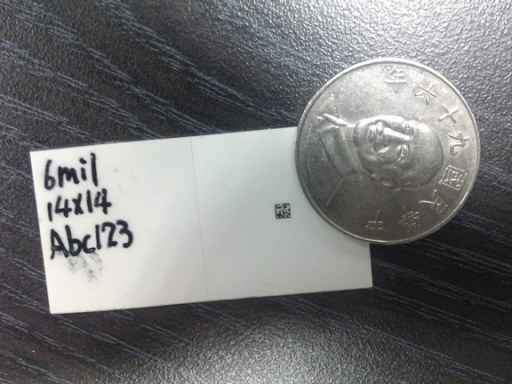
\includegraphics[width=0.4\linewidth]{smalldatamatrix.jpg}
	\caption{Comparando el tamaño de un datamatrix con una moneda.}
	\label{fig:datamatrixmoneda}
\end{figure}

El código Data Matrix utiliza entre un 30\% y un 60\% menos espacio que el código QR conteniendo los mismos datos. El tamaño mínimo es de 10x10 módulos, comparando el mínimo para el código QR es de 21x21 módulos. \cite{2006_Semacode_TECH_REPORT}
\\
El código GS1 DataMatrix, está basado en el estandar ECC200  por GS1 para su distribución y define reglas para diferenciarse del datamatrix tradicional. Se estandarizará en la industria médica, dado que deben imprimirse directamente en instrumentos médicos de acero, como cuchillos quirúrgicos y tijeras. En la versión ECC200, la cantidad de filas y columnas es siempre un número par. El máximo es de 144 filas y 144 columnas divididas en 36 regiones de datos de 22 filas y 22 columnas cada una. En cambio, el formato rectangular, la capacidad máxima es: 72 caracteres alfanuméricos, 98 números. \cite{GS12011}
